\section{Finite Element Models}
\label{FEMModels:sec}

\subsection{Overview}

\subsubsection{Structure}

\subsubsection{Materials}

\subsubsection{Boundary conditions}

\subsection{FEM model creation}

\subsubsection{Using factory methods}

\subsubsection{Using external meshes}

\subsubsection{Using direct code}

\subsubsection{A simple beam model}

\begin{figure}[h]
\begin{center}
\iflatexml
 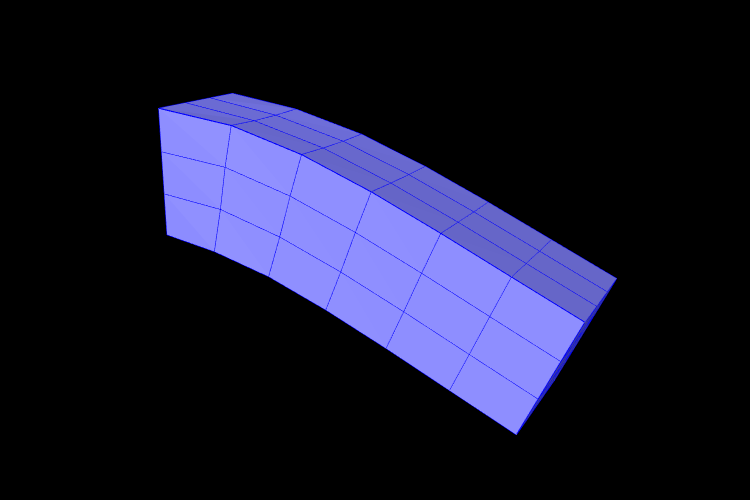
\includegraphics[]{images/FemBeam}
\else
 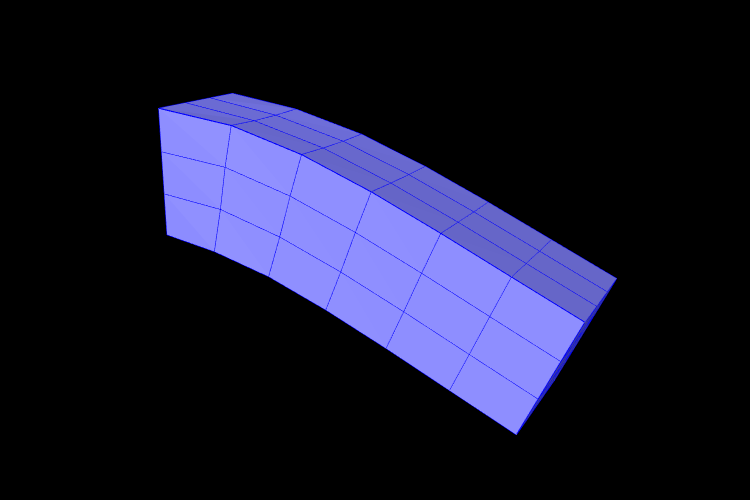
\includegraphics[width=3.75in]{images/FemBeam}
\fi
\end{center}
\caption{FemBeam model loaded into ArtiSynth.}
\label{FemBeam:fig}
\end{figure}

\subsection{FEM Geometry}

\subsubsection{Surface meshes}

\subsubsection{Embedding geometry within an FEM}

\subsubsection{A beam with an embedded sphere}

% EmbeddedFemSphere

\subsection{Node attachments}
\label{NodeAttachments:sec}

\subsubsection{General principles}

\subsubsection{Connecting a beam to a block}

\begin{figure}[h]
\begin{center}
\iflatexml
 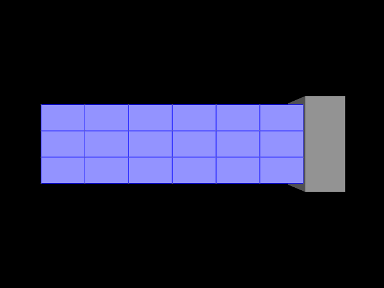
\includegraphics[]{images/FemBeamWithBlock}
\else
 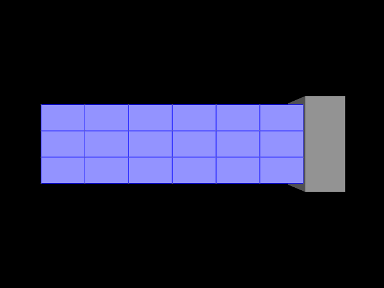
\includegraphics[width=3.75in]{images/FemBeamWithBlock}
\fi
\end{center}
\caption{FemBeamWithBlock model loaded into ArtiSynth.}
\label{FemBeamWithBlock:fig}
\end{figure}

% FemBeamWithBlock

\subsubsection{Connecting two FEMs together}

% ConnectedFems

\subsection{FEM markers}

\subsubsection{Embedding particles in FEMs}

\subsubsection{Attaching a FEM beam to a muscle}

\begin{figure}[h]
\begin{center}
\iflatexml
 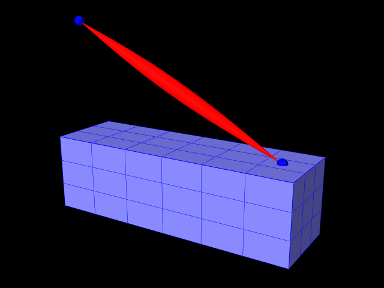
\includegraphics[]{images/FemBeamWithMuscle}
\else
 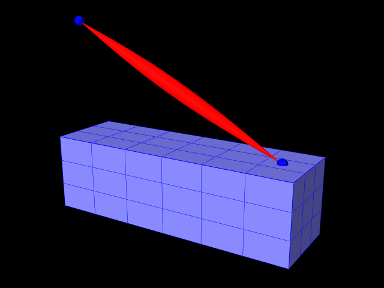
\includegraphics[width=3.75in]{images/FemBeamWithMuscle}
\fi
\end{center}
\caption{FemBeamWithMuscle model loaded into ArtiSynth.}
\label{FemBeamWithMuscle:fig}
\end{figure}

% FemBeamWithMuscle

\subsection{Muscle activated FEM models}

\subsubsection{FemMuscleModel}

\subsubsection{Activation with fibres}

\subsubsection{Activation with embedded materials}

\subsubsection{Comparision with two beam examples}

\begin{figure}[h]
\begin{center}
\iflatexml
 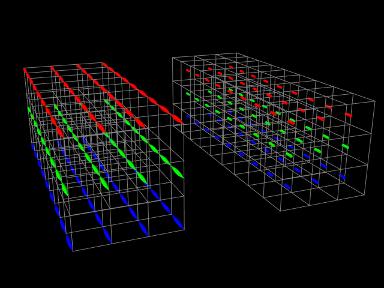
\includegraphics[]{images/FemMuscleBeams}
\else
 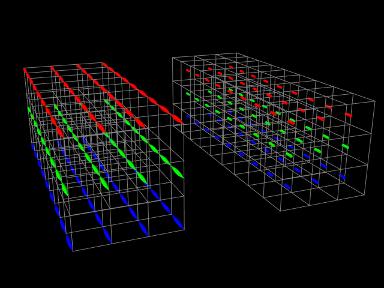
\includegraphics[width=3.75in]{images/FemMuscleBeams}
\fi
\end{center}
\caption{FemMuscleBeams model loaded into ArtiSynth.}
\label{FemMuscleBeams:fig}
\end{figure}

% FemMuscleBeams

\subsection{Collisions}

\subsubsection{Colliding with FEM geometry}

\subsubsection{Colliding with the surface mesh}

\begin{figure}[h]
\begin{center}
\iflatexml
 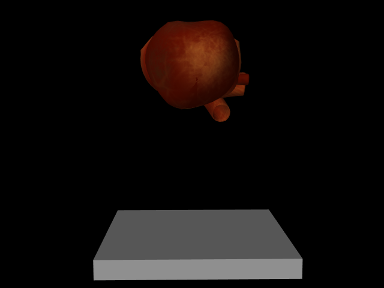
\includegraphics[]{images/FemMuscleHeart}
\else
 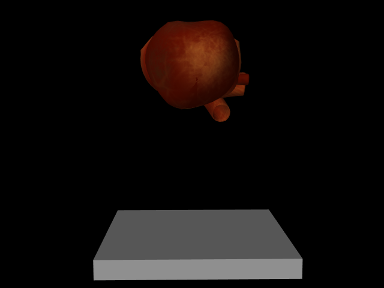
\includegraphics[width=3.75in]{images/FemMuscleHeart}
\fi
\end{center}
\caption{FemMuscleHeart model loaded into ArtiSynth.}
\label{FemMuscleHeart:fig}
\end{figure}

% FemMuscleHeart

\subsubsection{Colliding with an embedded sphere}

\begin{figure}[h]
\begin{center}
\iflatexml
 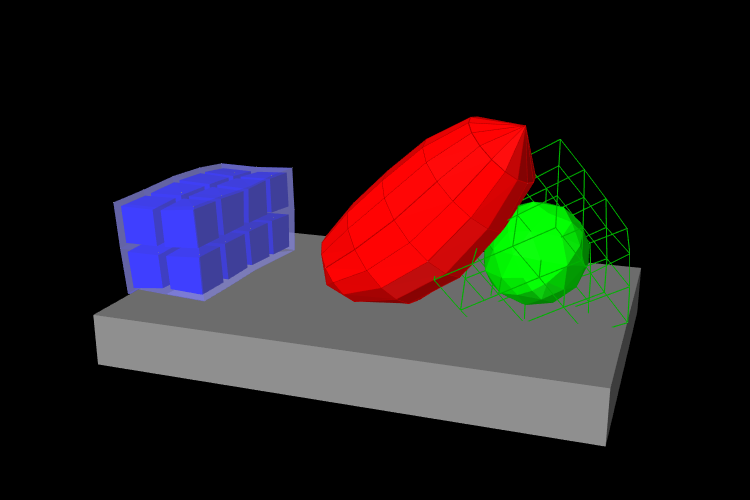
\includegraphics[]{images/FemCollisions}
\else
 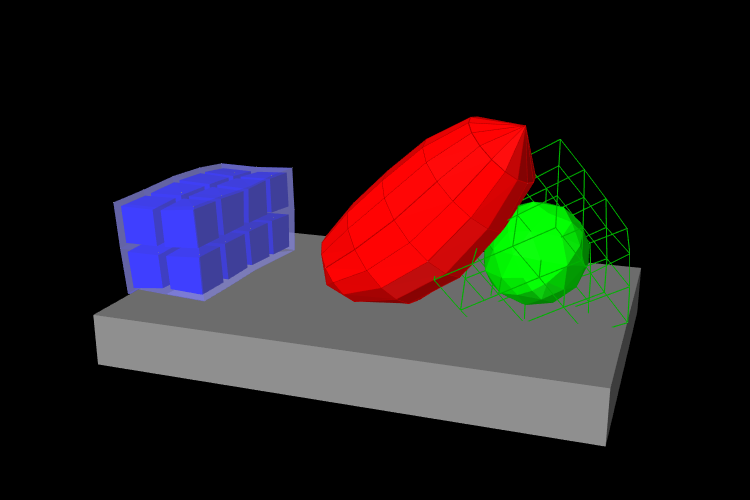
\includegraphics[width=3.75in]{images/FemCollisions}
\fi
\end{center}
\caption{FemCollisions model loaded into ArtiSynth.}
\label{FemCollisions:fig}
\end{figure}

\subsection{Visualization}

stuff stuff stuff

\subsubsection{Rendering settings}

stuff stuff stuff

\subsubsection{Stress and strain plotting}

stuff stuff stuff
